\documentclass[10pt,a4paper]{article}
\usepackage[utf8]{inputenc}
\usepackage{amsmath}
\usepackage{amsfonts}
\usepackage{amssymb}
\usepackage{graphicx}
\usepackage{hyperref}
\usepackage{caption}
\usepackage{subcaption}

\usepackage{listings}
\usepackage{color}

\definecolor{dkgreen}{rgb}{0,0.6,0}
\definecolor{gray}{rgb}{0.5,0.5,0.5}
\definecolor{mauve}{rgb}{0.58,0,0.82}

\lstset{frame=tb,
  language=Python,
  aboveskip=3mm,
  belowskip=3mm,
  showstringspaces=false,
  columns=flexible,
  basicstyle={\small\ttfamily},
  numbers=none,
  numberstyle=\tiny\color{gray},
  keywordstyle=\color{blue},
  commentstyle=\color{dkgreen},
  stringstyle=\color{mauve},
  breaklines=true,
  breakatwhitespace=true,
  tabsize=3
}


\begin{document}

%Proposal follows a well-organized structure and would be readily understood by its intended audience. Each section is written in a clear, concise and specific manner. Few grammatical and spelling mistakes are present. All resources used and referenced are properly cited.

\begin{titlepage}
	\centering
	\vspace{1cm}
	{\scshape\Large ED3S: Machine Learning Project \par}
	\vspace{1.5cm}
	{\huge\bfseries Image classification with PASCAL VOC dataset \par}
	\vspace{1.5cm}
	{\Large Author: Oscar Javier Hernandez\par}
	\vfill

% Bottom of the page
	{\large \today\par}
\end{titlepage}

\section{Definition}
%(approx. 1-2 pages)
\subsection{Project Overview}\label{sec: overview}
%In this section, look to provide a high-level overview of the project in layman’s terms. Questions to ask yourself when writing this section:
%
%Has an overview of the project been provided, such as the problem domain, project origin, and related datasets or input data?
%Has enough background information been given so that an uninformed reader would understand the problem domain and following problem statement?

\begin{itemize}
\item {\bf What problem is solved by your intended predictive model?}\\ 
The problem that I have chosen for my project is the object classification task using the Pascal VOC dataset. For the sake of time I focus on building classifier with four object categories; person, dog, cat, and car. I will outline the architectures of the implemented deep-neural networks that I trained for this purpose and discuss the data preprocessing steps that I took.

\item {\bf Why is it important to solve your particular problem?} \\
This particular problem is important to solve because it was numerous real-world applications. For example, self-driving cars use sophisticated algorithms and equipment to map out their environment, in order to take appropriate actions on the road, these cars need algorithms that can classify objects on-the-fly. If the classifier detects animals on the road, it will behave differently depending on the type of animal identified. Small animals, like cats and dogs may have a tendency to run into the road unexpectedly and so the car will drive more carefully than when the animals it identified are humans which are less prone to running onto the road. Of course the usefulness of this type of classifier is not limited to self-driving cars and can be used in other applications, which make this problem useful and important to solve.

\item {\bf How is the data representative of the learning problem?}\\
The PASCAL VOC dataset contains 9963 images, with 20 object classes in total. The four categories that I have chosen are are the subsets \lstinline{person,cat,dog,car}. The data is representative of the learning problem since 

\item {\bf How would the estimations of the model be used?}\\
The goal for this image classifier, in the case of the self-driving car example, would be for the self-driving vehicle to supply images via its cameras to the classifier, which will then return the object category to the vehicles computer on the fly. The algorithms in the vehicles computer system would then take the appropriate actions based on the results. However, in general the algorithms 
\end{itemize}
 

\newpage
\section{Analysis}
%(approx. 2-4 pages)

\subsection{Data Preprocessing}
%In this section, you will be expected to analyze the data you are using for the problem. This data can either be in the form of a dataset (or datasets), input data (or input files), or even an environment. The type of data should be thoroughly described and, if possible, have basic statistics and information presented (such as discussion of input features or defining characteristics about the input or environment). Any abnormalities or interesting qualities about the data that may need to be addressed have been identified (such as features that need to be transformed or the possibility of outliers). Questions to ask yourself when writing this section:
%
%If a dataset is present for this problem, have you thoroughly discussed certain features about the dataset? Has a data sample been provided to the reader?
%If a dataset is present for this problem, are statistics about the dataset calculated and reported? Have any relevant results from this calculation been discussed?
%If a dataset is not present for this problem, has discussion been made about the input space or input data for your problem?
%Are there any abnormalities or characteristics about the input space or dataset that need to be addressed? (categorical variables, missing values, outliers, etc.)

To load in the data, we used pandas to load the files:\\ 
\lstinline{person_test.txt,cat_test.txt,dog_test.txt,car_test.txt}\\
into a data frame where each row contains the image\_ID followed by values indicating whether the image contains a person, dog, cat or car (True = 1, False = -1). In addition we process the data and sure all of the objects in the dataframe are mutually exclusive. Therefore each image will belong to only one category. I performed this step to attempt to make the training process easier for the classifier, since it would be trained to produce only one unique class label  for each image during the training process. The first few entries of this dataframe are given below,
\begin{lstlisting}
   img_ID  is_person  is_dog  is_cat  is_car
0  002846          1      -1      -1      -1
1  002582          1      -1      -1      -1
2  004306         -1       1      -1      -1
3  001748          1      -1      -1      -1
4  005074         -1      -1      -1       1
...
\end{lstlisting}
After filtering the data to make the image categories mutually exclusive, the number of objects in each class are
\begin{lstlisting}
The total number of images:  2660
Number of Persons:  1619
Number of Dogs:  298
Number of Cats:  278
Number of Cars:  465
\end{lstlisting}

We notice that the category \lstinline{person} has significantly more objects than the other classes. During training, this may introduce a bias in our classifier and as a result of the large number of members in that category it may be better at detecting people than other objects. Therefore, to correct this problem, I choose to remove random images from the \lstinline{person} category until only 500 are left. Once this is complete, my code splits the remaining data set into 80$\%$ training and 20$\%$ validation sets. A bash script will then be generated that creates the \lstinline{testing, validation} folders which contain subfolders for each object category. The bash script will also place the appropriate copies of images into appropriate subfolders. Below I show an example of the new data frame, with the more balanced sets,
\begin{lstlisting}
=========================================
dropped:  1119
new person number:  500
new dog number:  298
new cat number:  278
new car number:  465
New Dataframe 1541
   img_ID  is_person  is_dog  is_cat  is_car
0  007342          1      -1      -1      -1
1  007001         -1      -1      -1       1
2  002821          1      -1      -1      -1
3  004874          1      -1      -1      -1
4  006394         -1      -1       1      -1
=========================================
\end{lstlisting}
After balancing and splitting into training/validation the total number of images that went these categories are 
\begin{lstlisting}
Training set size:  1233
Validation set size:  308
\end{lstlisting}
Because the image sets is still fairly small I used augmented images to generate more training samples from the data set. This was accomplished with the augmentation features in Keras in the following code snippet.

\begin{lstlisting}
train_datagen = ImageDataGenerator(
    rotation_range=50.,
    width_shift_range = 0.2,
    height_shift_range = 0.2,
    rescale=1. / scale,
    shear_range=0.2,
    zoom_range=0.2,
    horizontal_flip=True,
    vertical_flip = True
)


train_generator = train_datagen.flow_from_directory(
    train_data_dir,
    target_size=(img_width, img_height),
    batch_size=batch_size,
    class_mode='categorical')
\end{lstlisting}



\subsection{Algorithms and Techniques}
%In this section, you will need to discuss the algorithms and techniques you intend to use for solving the problem. You should justify the use of each one based on the characteristics of the problem and the problem domain. Questions to ask yourself when writing this section:
%
%Are the algorithms you will use, including any default variables/parameters in the project clearly defined?
%Are the techniques to be used thoroughly discussed and justified?
%Is it made clear how the input data or datasets will be handled by the algorithms and techniques chosen?
Because this is an image classification problem, I chose to use convolutional neural network architectures. 
For the architecture of the neural network I chose to try three different methods. The first is a simple benchmark model, consists of a convolutional network followed by a max pooling layer and then a dense layer with a softmax output. The summary of this network is below (Model 0),\\
\begin{lstlisting}
Model 0
_________________________________________________________________
Layer (type)                 Output Shape              Param #   
=================================================================
conv2d_24 (Conv2D)           (None, 254, 254, 32)      896       
_________________________________________________________________
activation_20 (Activation)   (None, 254, 254, 32)      0         
_________________________________________________________________
max_pooling2d_18 (MaxPooling (None, 127, 127, 32)      0         
_________________________________________________________________
flatten_10 (Flatten)         (None, 516128)            0         
_________________________________________________________________
dense_13 (Dense)             (None, 4)                 2064516   
_________________________________________________________________
activation_21 (Activation)   (None, 4)                 0         
=================================================================
Total params: 2,065,412
Trainable params: 2,065,412
Non-trainable params: 0
_________________________________________________________________
\end{lstlisting}

\newpage
The next network that we tried out (Model 1) was suggested in the Keras blog article \cite{Chollet_2016}
\begin{lstlisting}
Model 1
_________________________________________________________________
Layer (type)                 Output Shape              Param #   
=================================================================
conv2d_25 (Conv2D)           (None, 254, 254, 32)      896       
_________________________________________________________________
activation_22 (Activation)   (None, 254, 254, 32)      0         
_________________________________________________________________
max_pooling2d_19 (MaxPooling (None, 127, 127, 32)      0         
_________________________________________________________________
conv2d_26 (Conv2D)           (None, 125, 125, 32)      9248      
_________________________________________________________________
activation_23 (Activation)   (None, 125, 125, 32)      0         
_________________________________________________________________
max_pooling2d_20 (MaxPooling (None, 62, 62, 32)        0         
_________________________________________________________________
conv2d_27 (Conv2D)           (None, 60, 60, 64)        18496     
_________________________________________________________________
activation_24 (Activation)   (None, 60, 60, 64)        0         
_________________________________________________________________
max_pooling2d_21 (MaxPooling (None, 30, 30, 64)        0         
_________________________________________________________________
flatten_11 (Flatten)         (None, 57600)             0         
_________________________________________________________________
dense_14 (Dense)             (None, 64)                3686464   
_________________________________________________________________
activation_25 (Activation)   (None, 64)                0         
_________________________________________________________________
dropout_11 (Dropout)         (None, 64)                0         
_________________________________________________________________
dense_15 (Dense)             (None, 4)                 260       
_________________________________________________________________
activation_26 (Activation)   (None, 4)                 0         
=================================================================
Total params: 3,715,364
Trainable params: 3,715,364
Non-trainable params: 0
_________________________________________________________________
\end{lstlisting}

\newpage
\noindent
The third model that we will use is the VGG-like convnet suggested in \cite{KerasDocs}:
\begin{lstlisting}
Model 2
________________________________________________________________
Layer (type)                 Output Shape              Param #   
=================================================================
conv2d_46 (Conv2D)           (None, 256, 256, 32)      896       
_________________________________________________________________
conv2d_47 (Conv2D)           (None, 254, 254, 32)      9248      
_________________________________________________________________
max_pooling2d_31 (MaxPooling (None, 127, 127, 32)      0         
_________________________________________________________________
dropout_24 (Dropout)         (None, 127, 127, 32)      0         
_________________________________________________________________
conv2d_48 (Conv2D)           (None, 127, 127, 64)      18496     
_________________________________________________________________
conv2d_49 (Conv2D)           (None, 125, 125, 64)      36928     
_________________________________________________________________
max_pooling2d_32 (MaxPooling (None, 62, 62, 64)        0         
_________________________________________________________________
dropout_25 (Dropout)         (None, 62, 62, 64)        0         
_________________________________________________________________
conv2d_50 (Conv2D)           (None, 62, 62, 64)        36928     
_________________________________________________________________
conv2d_51 (Conv2D)           (None, 60, 60, 64)        36928     
_________________________________________________________________
max_pooling2d_33 (MaxPooling (None, 30, 30, 64)        0         
_________________________________________________________________
dropout_26 (Dropout)         (None, 30, 30, 64)        0         
_________________________________________________________________
flatten_15 (Flatten)         (None, 57600)             0         
_________________________________________________________________
dense_22 (Dense)             (None, 512)               29491712  
_________________________________________________________________
dropout_27 (Dropout)         (None, 512)               0         
_________________________________________________________________
dense_23 (Dense)             (None, 4)                 2052      
=================================================================
Total params: 29,633,188
Trainable params: 29,633,188
Non-trainable params: 0
_________________________________________________________________
\end{lstlisting}

\newpage
\section{Results}
 In Fig.~\ref{fig: Final results 128} I plotted the results of training all three models. 

\begin{figure}[h]
\centering
\begin{subfigure}{.7\textwidth}
  \centering
  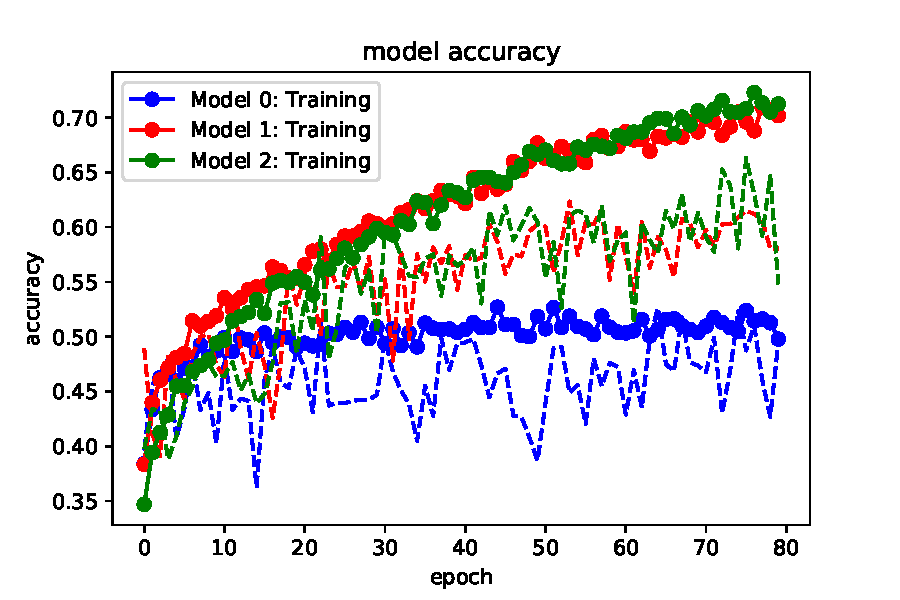
\includegraphics[scale=0.5]{accuracy_vs_epoch_128.pdf}
  \caption{The accuracy of the model vs epoch for\\ three models.}
  \label{fig:sub1 128}
\end{subfigure}%
\begin{subfigure}{.6\textwidth}
  \centering
  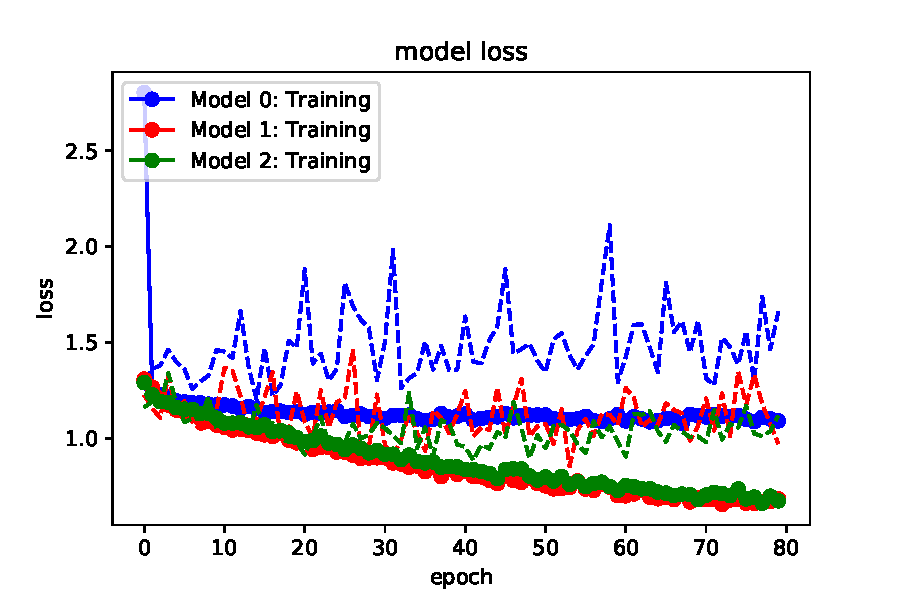
\includegraphics[scale=0.5]{loss_vs_epoch_128.pdf}
  \caption{The loss of the model vs epoch for\\ the three models.}
  \label{fig:sub2 128}
\end{subfigure}
\caption{The results for three models using \lstinline{scale=128} factor}
\label{fig: Final results 128}
\end{figure}


\begin{table}[h]
\centering
\begin{tabular}{cccccl}
Model & Training Accuracy & Training Loss & Validation Accuracy  & Validation Loss & scale \\ \hline
0 & 0.5  & & 0.45 & & 128    \\
0 & -  & & - & & 256    \\
1 & 0.7  & & 0.56 & & 128   \\
1 & -  & & - & & 256    \\
2 & 0.7  & & 0.56 & & 128 \\
2 & -  & & - & & 256    \\
\end{tabular}
\caption{The accuracy and losses for the training and validation sets for the three different models.}
\end{table}


\subsection{Challenges}
This project had many challenges associated with it. The first problem that I encountered was that many of the images had multiple objects in it. To fix this problem, I separated the images into mutually exclusive sets. I also tried at one point to use an ``other" category for objects that the network didn't recognize, but this didn't work on the network. I decided to drop this extra category. Another issue was that some of the categories that I tried to train the networks on didn't have enough data, for example, there were only roughly ~50 images of cows, so I was not able to use this category. The categories that were used in this project were the ones I found that had the largest number of mutually exclusive members but it took some time to figure this out. Another problem that I encountered was slow execution times on CPUs, when I first developed this code, I was running it on my laptop but this proved too slow until I moved the code onto a Kaggle Kernel with a GPU, however, training the three models still takes time.


\newpage
\subsection{Outlook}
The best achieved accuracy for the models that we constructed were only $70 \%$. This unfortunately is lower that I expected but in the future, I would like to extend the networks I implemented by using deeper neural networks with different hyperparameters. 

\begin{thebibliography}{9}

\bibitem{Chollet_2016}
F. Chollet, (2016), ``Building powerful image classification models using very little data" \url{https://blog.keras.io/building-powerful-image-classification-models-using-very-little-data.html} [Accessed 29 Jul. 2018].
\bibitem{KerasDocs} ``Getting started with the Keras Sequential model" \url{https://keras.io/getting-started/sequential-model-guide/#examples}[Accessed 29 Jul. 2018].


\end{thebibliography}
\end{document}